\chapter{Datasets for Separation and Analysis}
\label{cha:datasets}
In the previous chapter various applications and problems in the context of highly overlapped signals were discussed.
Before methods are presented that separate or analyze such signals are presented, it is helpful to study and understand the importance of data with these properties.
This becomes especially important as many methods nowadays rely on machine learning algorithms.
One of the objectives in this thesis is to discuss its modulation properties of the signals can be used as a cue for the signal.
Even though modulation is an apparent property of many audio recordings such as speech and music, very vew dataset are available to actually study influence of the modulation into various tasks such as source separation.
\par
In speech, it is very wide spread to mix clean speech and noise~\cite{varga93}or different clean speech signals like~\cite{garofolo93} to generate mixed speech.
It is known that the conversational aspect is lost here but it may not be that important.
Now, the benefit of such a dataset is that it can easily get very large.
In music however, recordings are typically available separated.
That way only very few datasets exist with separated tracks. This
% zafar
Compared to speech, musical content usually does share common orchestration and can usually not superimposed in a random way, prohibiting simply summing isolated random notes from instrumental databases to produce mixtures.
% zafar end

\begin{itemize}
  \item Monophonic vs. Polyphonic
  \item Live Recordings vs. Studio Recordings
  \item Real instruments vs. synthetic instruments
\end{itemize}

\section{Synthetic Datasets}

\emph{TODO!}

To create a dataset of synthetic mixtures of high overlap, one would seek for a high quality.

The simplest way to assemble overlapped data is to use individual audio recordings and randomly mix them together.
% * Am einfachsten durch verwendung existierender Einzelaufnahmen und anschliessender Überlagerung
However, this often does not maintain the realistic behavior of mixtures.

For example, it is known that a mixture of random speakers does not assemle a realistic cocktail party nor a conversation.

Comparing this to music would mean, mixing individual sigle notes. But transforming this into music would require a composition including notes.

Für kleiner Datensets eignet sich

A) synthetisierung von Noten MIDIs (partituren) zu synthetisieren zum die volle Kontrolle zu haben (RWC in Kapitel X)
B) Remixing von existierenden multitrack Datensets (medleydb). DSD100, MUSDB

Möglichkeit um schnell viele samples zu erstellen: zufällige überlagerung.

Clou: es gibt nur ein einziges musikalisches szenario bei dem zwei zufällige instrumente zusammengemischt werden können.. Unisono.

Zwei Erklärungen:

1. zufällige Überlagerung von verschiedenen Instrumenten ist nur musikalisch "sinnvoll" wenn gleicher Ton.
2. auch musikalisch verwendung in klassischer Musik zur Erweiteurng des timbre.
3. zeitlicher onset nicht relevant (unisono funktioniert nicht mit perkussiven Instrumenten)

Nehme man jetzt zwei echte Aufnahmen gleicher Töne unterschiedlicher ergeben sich jedoch folgende Probleme:

A) nicht exakt gleiche Tonhöhe (eventuell auch durch unterschiedliche Stimmung (Kammerton!))
B) Kein kontrolliertes Vibrato
C) unterschiedliche akustische umgebungen (Raumakustik etc.)

>> Synthetisch....

Bei Sprache ist die zufällige Zusammenmischung kein so grosses Problem. Ein realistisches Cocktail party effekt tritt bereits mit zufälliger Überlagerung ein. Nachteil: Keine semantischen Dialoge. Effekt nicht untersucht (paper zitieren.)

Fazit

+ Controlled Environments
+ Allows to check parameters
+ Reproduzierbarkeit
+ "Handlich"
- Eventuell Nicht übertragbar
- Overfitting

* synthetic Datasets: unison source separation Chapter{X}
* Dafx paper und commonfate paper
libri speech, RWC (midified)

\subsection{Unison Instrument Scenario}
\label{sec:scenario}

% TODO: True Unison would be if 2 violins perceived as a single source, and usually there is no need to separate their signals from each other.

% from common fate introduction
When St\"oter and Schoeffler et. al. \cite{stoeter13, schoeffler13} asked participants to identify the number of instruments in a piece of music, the participants were only able to identify up to three, similar to Huron's voice experiments. There is very little chance that listeners are able to detect the presence of more than three sources. However in trials with fewer than three instruments, listeners tended to be very sensitive: One of the stimuli in the \cite{stoeter13, schoeffler13} experiments with 1168 participants consisted of a mixture of Violin and Flute played in unison. The results showed that $76\%$ of the participants correctly identified two instruments. Only $18\%$ of the participants underestimated by one instrument, $6\%$ overestimated by one instrument.

Since humans are able to reliably detect even instruments played in unison, this is a good motivation to expect the same from an algorithm. In this paper we want to address this scenario which has not been brought up so far. We believe creating and evaluating new algorithms for separating sources playing in unison will improve source separation systems in general.

% TODO: unison source separation scenario, aber wohin mit dem datenset?
We propose a scenario where instruments play in unison. This means that they share the same fundamental frequency (regardless of the octave) so that the sources can overlap both in time and frequency. In fact unison\footnote{greek: with \emph{one voice}} mixtures are meant to be as much overlapped as possible, hence they are very difficult to separate. However, due to masking effects, a relatively good subjective quality for the separated sources can be obtained, even if the other sources are not perfectly suppressed.
As far as we know, there is no contribution to the source separation scene that focuses on mixtures of such unison sources. \\

% TODO: Extend this
True Unison would be if 2 violins perceived as a single source, and usually there is no need to separate their signals from each other.

The items have each been generated by rendering C4 notes in a state of the art software sampler. All test have a duration of about three seconds. Items were equalized in loudness by using an iterative calculation of the loudness algorithm of the time varying Zwicker model. The implementation \cite{genesis12} was used. The 10 instrument items then generated 45 unique mixtures of two instruments each. The processing was done in 44.1~kHz / 16 bit.

\begin{table}
\begin{center}
\footnotesize
\begin{tabular}{ l l l}
  Instrument & Vibrato &  General MIDI \# \\
  \hline
  Violin & yes & 40 \\
  Viola & yes & 41 \\
  Violon Cello & yes & 42 \\
  Trumpet & no & 56 \\
  Trombone & no & 57\\
  Horn & no & 60  \\
  Bariton Sax & yes & 67 \\ % TODO
  Oboe & no & 68\\
  Clarinet & no & 71\\
  Flute & yes & 73\\
\end{tabular}
\end{center}
\caption{Instrument item test set}
\label{tab:testset}
\end{table}

\section{Realistic Data}

\subsection{Single Note Data}

\begin{figure}[h]
  \centering
  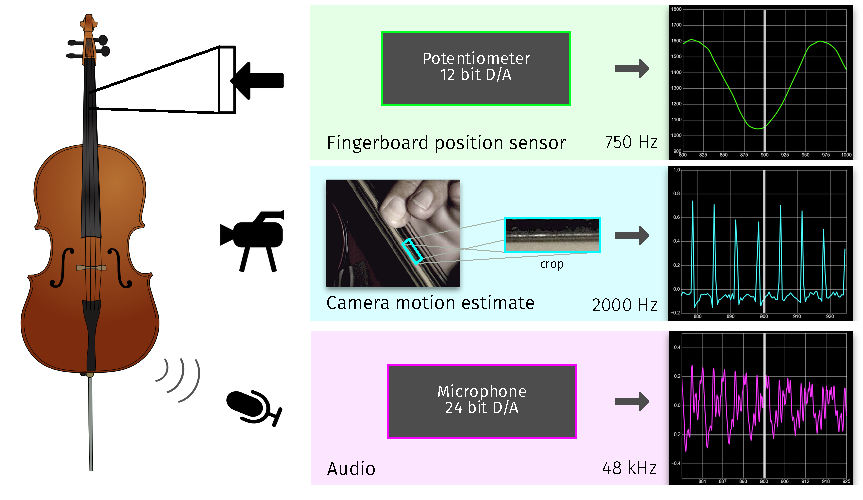
\includegraphics[width=\textwidth]{Chapters/04_Data/figures/teaser.pdf}
  \caption{Overview of the multi-modal data recorded for the proposed dataset.}
\label{fig:teaser}
\end{figure}

% from
Estimating the fundamental frequency ($F0$) of a signal is a well studied task in audio signal processing with many applications. If the $F0$ varies over time, the complexity increases, and it is also more difficult to provide ground truth data for evaluation.
Besides audio data, we include sensor recordings capturing the finger position on the fingerboard which is converted into an instantaneous frequency estimate. In speech processing, the electroglottograph (EGG) is able to capture the excitation signal of the vocal tract, which is then used to generate a reference instantaneous $F0$.
Inspired by this approach, we included high speed video camera recordings to extract the excitation signal originating from the moving string.
In the proposed test set we chose the violin cello for the following reasons: (1) vibrato is used as a common style for expression, (2) there is an observable physical relationship between frequency modulation and vibrato, and (3) the instrument is large enough to embed sensors to capture the vibrato. The properties of the cello are studied by research in acoustics~\cite{woodhouse2004bowed, woodhouse1999torsional}.
The aim of the multi-sensor recordings is to capture the major aspects of the cello while being played by a musician. We identify three main components: (1) The excitation caused by the moving bow; (2) the vibrating string, and (3) the finger, controlling the string length by rolling it on the fingerboard.
The main focus of the recordings is set to analyze vibrato playing style. Since it is common that vibrato characteristics differ from musician to musician, all recordings were performed by two musicians. One is a professional cellist with 30 years of experience in a symphonic orchestra. The other musician is an amateur with less than 1 hour per week of practice. The recordings took place on a single day and were conducted on a mid-quality full-size cello equipped with sensors as described below. Due to the width of fingerboard sensors and the attached cables we were able to equip two strings (G and A) allowing to record pitches ${G2, D3, D^\sharp3, E3, A3, B3, C4, C^\sharp4}$ from both musicians. The resulting test set yields in $148$ recorded notes after removal of some notes due to errors in the sensor recordings. The process for cleaning up the data is documented\footnote{\url{https://github.com/audiolabs/muserc}}. The dataset is released under a Creative Commons license.

\subsection{Multitrack Data}

The Signal Separation Evaluation Campaign (SiSEC) is a solid indicator of the progress in research within the field of source separation \cite{vincent12}. The results from 2013 \cite{sisec13} show that for professionally produced music it is still difficult to achieve a high quality separation.
One reason is due to the fact that the wide use of non-linear post-processing techniques (e.g. dynamic compression or effects like reverb) break assumptions that often are required to enable good performance of source separation algorithms. Another reason is that non-stationary effects like vibrato introduce additional problems \cite{nakano10}.

Multitrack datasets are helpful to develop and evaluate methods.

* real world datasets: , SiSEC16, SiSEC18,

* throughout the thesis: how to go from synthetic to real world datasets if available.

% zaffar begin
Building a good data-driven method for source separation relies heavily on a training dataset to learn the separation model. In our case, this not only means obtaining a set of musical songs, but also their constitutive accompaniment and lead sources, summing up to the mixtures. For professionally-produced or recorded music, the separated sources are often either unavailable or private. Indeed, they are considered amongst the most precious assets of right holders, and it is very difficult to find isolated vocals and accompaniment of professional bands that are freely available for the research community to work on without copyright infringements.
% zafar end

% from dafx
Audio source separation is a very active research field with a large number of contributions. Applications are dependent on the context of the scenario, ranging from enhancements of speech signals to musically motivated analysis tasks.

As outlined by Bregman~\cite{bregman94}, the human ability to detect and group sound sources is outstanding.

% TODO Listing more application (get from commonfate)
The separation of musical instruments from a single channel mixture is considered as an under-determined case which does not have a single solution. Knowing the way in which source signals are mixed together is crucial to the quality of separation systems. In the context of speech separation even unsupervised methods can lead to good results. This is due to the fact that mixtures of speech signals (like in a cocktail party environment) show a high degree of statistical independence. Mixtures of musical instruments, however, are highly correlated which is a desired aim of musical performances in general.

In the following years, new datasets were proposed that improved over the MASS dataset in many directions. We briefly describe the most important ones, summarized in Table~\ref{tab:datasets}.
\begin{itemize}[leftmargin=*]
	\item The QUASI dataset was proposed to study the impact of different mixing scenarios on the separation quality. It  consists of the same tracks as in the MASS dataset, but kept full length and mixed by professional sound engineers.
	\item The MIR-1K and iKala datasets were the first attempts to scale vocals separation up. They feature a higher number of samples than the previously available datasets. However, they consist of mono signals of very short and amateur karaoke recordings.
	\item The ccMixter dataset was proposed as the first dataset to feature many full-length stereo tracks. Each one comes with a vocals and an accompaniment source. Although it is stereo, it often suffers from simplistic mixing of sources, making it unrealistic in some aspects.
	\item MedleyDB has been developed as a dataset to serve many purposes in music information retrieval. It consists of more than 100 full-length recordings, with all their constitutive sources. It is the first dataset to provide such a large amount of data to be used for audio separation research (more than 7 hours). Among all the material present in that dataset, 63 tracks feature singing voice.
  \item DSD100 was presented for SiSEC 2016. It features 100 full-length tracks originating from the 'Mixing Secret' Free Multitrack Download Library\footnote{\url{http://www.cambridge-mt.com/ms-mtk.htm}} of the Cambridge Music Technology, which is freely usable for research and educational purposes.
\end{itemize}

In any case, it can be seen that datasets of sufficient duration to build data-driven separation methods were only created recently.

\begin{table*}[htbp]
	\centering
	\caption{Summary of datasets available for lead and accompaniment separation. Tracks without vocals were omitted in the statistics.}
	\label{tab:datasets}
		\begin{tabular}{l l l l l l}
			\hline
			\textbf{Dataset} & \textbf{Year} & \textbf{Reference(s)} & \textbf{Tracks} & \textbf{Track duration (s)} & \textbf{Full/stereo?}\\
			\hline
			MASS & 2008 & \cite{MTGMASSdb} & 9 & $16 \pm 7$ & no / yes \\
			MIR-1K & 2010 & \cite{hsu10} & 1,000 & $8 \pm 8$ & no / no \\
			QUASI & 2011 & \cite{liutkus11,vincent12} & 5 & $206 \pm 21$ & yes / yes \\
			ccMixter & 2014 & \cite{liutkus142} & 50 & $231 \pm 77 $ & yes / yes \\
			MedleyDB & 2014 & \cite{bittner14} & 63 & $206 \pm 121$ & yes / yes \\
			iKala & 2015 & \cite{chan15} & 206 & 30 & no / no \\
			DSD100 & 2015 & \cite{ono15} & 100 & $251 \pm 60$ & yes / yes \\
      MUSDB18 & 2017 & \cite{rafii17} & 150 & $236 \pm 95$ & yes / yes \\
			\hline
		\end{tabular}
\end{table*}
